
В этом документе описываются важные подробности о предстоящем событии генерации токена ASR (TGE), назначении токена ASR и юридических требованиях для участия в ASR TGE. Так же планируются, первоначальное предложение по обмену (IEO) и первоначальное предложение по децентрализованному обмену (IDO).

\section{TGE}
ASR TGE будет проведено в два этапа. Первый этап состоится в середине 2019 года. Второй этап состоится позже в 2019 году. Токены совместимы с ERC20 и ограничены предложением в 100.000.000. В общей сложности мы продадим 45 \% всех служебных токенов ASR («ASR») через TGE.
\newline\newline
Github: \url{https://github.com/AsureNetwork/crowdsale}

\newpage

\section{Детали TGE}

\begin{table}[H]
\begin{tabular}{lp{.6\textwidth}l}
  Имя токена (Ticker) & Asure (ASR) \\  
  Эмитент токена & Asure Foundation, Цуг, Швейцария\\
  Тип токена & ERC20\\
  Общее колличество токенов & 100.000.000 ASR \\
  Токены для публичной продажи & 45.000.000 ASR \\
  Токены для баунти кампании & 5.000.000 ASR \\
  Принимаемая валюта & ETH \\
  Курс обмена & 1 ASR = \$ 1.00 (эквивалент ETH) \\
  Минимальный вклад & 0.5 ETH \\\hline  
 
  Предпродажа & 1 Августа, 2019 | 15 Августа, 2019 \\
%19\textsuperscript{th} Feb - 12\textsuperscript{th} Mar 2019 \\
  Кап предпродажи & \$ 5.000.000 | 10 миллионов ASR\\
  Условия предпродажи & Первая неделя 50\% бонус (\$ 0.50) \newline
                  После первой недели 25\% бонус (\$ 0.75)\\\hline
  
  Основная продажа & 1 Декабря, 2019 | 31 Декабря, 2019 \\
%13\textsuperscript{th} Sep - 25\textsuperscript{th} Dec 2019 \\  
  Кап основной продажи & \$ 35.000.000 | 35 миллионов ASR\\
  Условия основной продажи & Первая неделя 15\% бонус (\$ 0.85)*\newline
                    Посе первой недели 0\% бонус (\$ 1.00)*\\\hline

%Special Bonus & 
%From \$ 5 to \$ 25 thousand  5\%\newline
%From \$ 25 thousand 10\%\\\hline

  Ограничение торговли токенами & Только команда и советники имеют периоды блокировки вложений и продаж. \\
  Листинг & ASR токены будут размещены на криптобиржах. \\\hline     

%Token Holder Benefits & 
%ASR token serves as the access to the Asure network by\newline
%\textbf{Network Validators:} Block rewards\newline
%\textbf{Service Providers:} Service rewards\\
  
  Хардкап & \$ 40.000.000
  
\end{tabular}
\caption{\label{tab:table-name}Детали токена}
\end{table}

* На планируемый курс может повлиять развитие цен на биржах. Обменный курс устанавливается один раз перед каждой фазой продажи и не будет изменен во время фазы продажи.

\section{Токен}

Токен ASR является служебным токеном. Он реализован в виде смарт-контракта Ethereum и поддерживает стандарты токенов ERC-20. Токен будет использоваться сетевыми валидаторами, а также поставщиками услуг для участия в качестве держателей в механизмах согласования proof-of-stakes в сети Asure. Это стимул работать правильно. Кроме того, токен ASR будет использоваться для управления сетью Asure.

\begin{figure}[H]
    \centering
    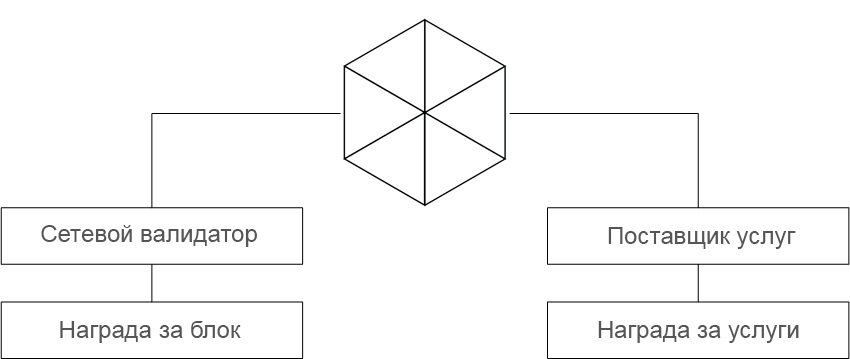
\includegraphics[width=4.0in]{img/staking.png}
    \caption{Что является преимуществом для держателей наших токенов?}
    \label{fig:asure_architecture}
\end{figure}

\textbf{Сетевые валидаторы:}
Для проверки транзакций в Сети Azure сетевым валидаторам необходимо иметь долю от поставляемого количества токенов ASR. В свою очередь, сетевые валидаторы получают плату за транзакции сети в виде токенов ASR, в качестве стимула для проверки правильности блоков. В случае мошеннического поведения валидатора, этот мошеннический валидатор теряет свою долю в сети.\newline

\textbf{Поставщики услуг:}
Токен ASR служит стимулом для правильной работы поставщиков услуг на платформе Asure и в соответствии с их объявлениями в рамках SLA. Поставщики услуг должны внести депозит в виде токенов, которые сохраняются в случае несоблюдения соответствующего SLA. Сервисом в сети Asure может быть например, оракулы, продукты, перестрахование и деятельность по продажам.\newline

Спрос на токены ASR будет создаваться двумя следующими механизмами: С ростом сети и платформы Asure все больше сетевых валидаторов и поставщиков услуг будут вынуждены стакать токены ASR. Чем больше сетевые валидаторы и поставщики услуг хотят заработать, тем больше необходимо токенов ASR.\newline
Токен ASR будет размещен на криптообменниках для публичной торговли, чтобы поставщики услуг сети, блокчейна или платформы Asure могли покупать и продавать токены ASR.\newline

\textbf{Управление:}
Управление On-Chain имеет решающее значение. Владельцы токенов ASR смогут управлять блокчейном Asure, сетью и голосовать за будущие улучшения.
\newline

\section{Ценность токена}
Основным фактором, влияющим на цену токена ASR, является спрос со стороны экосистемы, в которой токен может быть использован в механизмах достижения консенсуса в отношении доказательств заинтересованности и управления сетью. Asure уже разработал несколько сценариев приложений и нуждается в масштабируемой сети для устойчивой работы. Системы социального обеспечения вызывают большие объемы транзакций. При использовании токенов ASR для оплаты транзакций в сети увеличивается спрос на токен ASR и следовательно стоимость токена тоже.


\section{Распределение токенов}

Важно, чтобы сообщество понимало, как средства будут инвестироваться в будущем для создания сети социального обеспечения. Смотрите ниже, как будут распределены инвестиции.

\begin{itemize}
\item \textbf{Этап 1:} 55\% всех токенов ASR будет сгенерировано.
\item \textbf{Этап 2:} 45\% всех токенов ASR будет сгенерировано.
\end{itemize}

\newpage \subsection{Этап 1}

На первом этапе 20\% всех токенов ASR будет сгенерировано.

\begin{table}[H]
\begin{tabular}{llp{.62\textwidth}l}
  10\% & Публичная предпродажа & Вклады будут использоваться для разработки минимально жизнеспособного продукта сети и для создания более широкого сообщества.\\
  5\% & Семья и Друзья & Семья и Друзья получат свои токены как часть своего компенсационного пакета.\\
  5\% & Баунти & Asure обеспечивает компенсацию за ряд задач, распределенных между маркетингом, отчетами об ошибках или даже улучшением аспектов сети, блокчейна и платформы Asure.\\
  35\% & Фонд & Содержит инициативы по развитию и обучению основ, стимулы для разработчиков и исследования блокчейна, масштабирования, сети и платформы.
\end{tabular}
\caption{\label{tab:table-name} Этап 1 - Распределение токенов}
\end{table}

\textbf{Hint:} Все непроданные токены Этапа 1 (Предпродажа) будут перенесены на Этап 2 (Основная продажа).

\newpage

\subsection{Этап 2}

На втором этапе будет распределено 80\% всех токенов ASR.

\begin{table}[H]
\begin{tabular}{llp{.62\textwidth}l}
  35\% & Публичная основная продажа & Взносы будут использованы для разработки платформы, а также для финансирования безопасности, юридических и оперативных потребностей. \\
  8\% & Команда  & Они размещены для подтверждения времени, усилий и ресурсов, внесенных в платформу Asure. Команда Asure получит свои токены как часть своего компенсационного пакета.\\
  2\% & Консультанты & Консультанты получают свои токены как часть своего компенсационного пакета.
\end{tabular}
\caption{\label{tab:table-name} Этап 2 - Распределение токенов}
\end{table}

\textbf{Hint:} Все непроданные токены Этапа 2 (Основная продажа) TGE  будут сожжены.

\subsection{Первоначальное Предложение Обмена (IEO)}
Первоначальное предложение обмена предлагает множество преимуществ для всех вовлеченных сторон:

\textbf{Со стороны инвесторов:}
Инвесторы доверяют проверенной бирже, которую они уже знают.
Инвесторам не придется переплачивать за газ, так называемая "газовая война" будет предотвращена.
Многие уже зарегистрированы на биржах.

\textbf{Со стороны бирж:}
Новым клиентам и трейдерам необходимо зарегистрироваться на бирже, если у них еще нет учетной записи. Дополнительные источники дохода инвесторов.

\textbf{Со стороны Asure Network:}
Биржа имеет гораздо более широкую базу клиентов и следовательно, больше потенциальных инвесторов.
Доверие инвесторов к предполагаемой бирже выше, чем к новому блокчейн-проекту.
Листинг на бирже является следующим естественным шагом после пердложения токенов. Наконец, токен должен стать торгуемым для трейдеров.
\newline\newline
По этим причинам мы заинтересованы в том, чтобы оставаться гибкими и предоставлять токены ASR для IEO в любой точке краудсейла, сохраняя при этом значение общего предложения постоянным и не создавая дополнительных токенов. В сотрудничестве с партнерами по IEO, согласованное количество токенов ASR будет передано соответствующим партнерам из краудсейл-контракта.

\subsection{Вестинг}
В соответствии с передовой практикой и для защиты инвесторов и будущих участников нашей платформы, мы заблокируем токены нашей команды и консультантов. Команда и консультанты Asure получат свои токены в течение двух лет после начала второго этапа.
Вестинг гарантирует стабильность курса и приверженность всех вовлеченных членов. Если владелец попытается передать больше токенов ASR, чем получено, транзакция будет заблокирована.
Мы собираемся опубликовать смарт контракт на управление передачей прав в рамках нашего проекта. Следовательно, мы докажем сообществу нашу долгосрочную приверженность.
\newline\newline
Github: \url{https://github.com/AsureNetwork/crowdsale}

\newpage \section{Распределение средств}

Мы предполагаем, что все ETH полученные от продажи токенов ASR, будут распределены следующим образом:
\newline\newline

\begin{table}[H]
\begin{tabular}{llp{.6\textwidth}l}
  40\% & Платформа R\&D & Создание постоянного развития нашей сети уровня 2 \\
  25\% & Налоги & Налоги и плата за организацию развития.\\
  20\% & Маркетинг и Операции & Дополнительный персонал и ресурсы для повседневной работы и разумного управления по мере расширения организации. \\
  10\% & Правовой сектор & Мы остро осознаем необходимость неукоснительного соблюдения. Нам потребуется наша собственная хорошо обеспеченная правовая поддержка. Наша главная задача состоит в том, чтобы вписаться в сложные нормативные рамки по всему миру, чтобы сделать рост сообщества юридически безопасным. \\

  5\% & Офисные расходы & Офисные расходы и кадровая деятельность для формирования команды для достижения целей дорожной карты
\end{tabular}
\caption{\label{tab:table-name}Распределение средств}
\end{table}

\newpage 

\section{KYC/AML}

Основная цель регистрации продажи токенов, это обеспечить обязательную проверку "Знай своего клиента" (KYC) для предотвращения кражи личных данных, финансирования терроризма, борьбы с отмыванием денег (AML) и финансовым мошенничеством. Это также позволяет нашей команде лучше понимать наших держателей токенов и соответствующим образом управлять возможными рисками.

Токены ASR не предлагаются и не распространяются, а также не могут быть перепроданы или иным образом отчуждены их владельцами гражданам, физическим и юридическим лицам, имеющим свое обычное место жительства, место нахождения или место регистрации в стране или на территории, где операции с цифровыми монетами запрещены или каким-либо образом ограничены применимыми законами или правилами, или будут запрещены или ограничены в любое время после вступления в силу настоящего Соглашения (“ограниченные лица”).

Мы не принимаем участие от ограниченных лиц и оставляем за собой право отказать или отменить заявки на покупку токенов ASR в любое время по нашему собственному усмотрению, когда информация, предоставленная покупателями в рамках процедуры KYC, недостаточна, неточна или вводит в заблуждение или покупатель считается ограниченным лицом.

\section{Белый список}

Участие в TGE возможно только для участников из белого списка, которые выполнили процесс KYC.
\newline\newline
KYC: \url{https://www.asure.network/kyc/}

\section{Конфиденциальность и Безопасность}
Безопасность ваших данных очень важна для нас. Когда дело доходит до безопасности, нет «острых углов», даже под причинами запуска TGE. Поэтому, пожалуйста, ниже вы сможете найти меры, которые будут применяться для обеспечения вашей конфиденциальности и безопасности:

Asure никогда не будет передавать личные данные участников третьим лицам без предварительного согласия. Чтобы быть в безопасности, вы должны принять следующие меры предосторожности:

Никогда не отправляйте фиатные деньги или крипто-монеты на любой адрес во время регистрации. Существует только одна публичная дата продажи токенов, и она указана на нашем веб-сайте: https://www.asure.network. Добавьте в закладки веб-сайт регистрации и никогда не переходите по нему по ссылкам электронной почты.
Никогда не доверяйте электронным письмам, связанным с конкретными деталями продажи (такими как информация о софт или хардкапе, адрес Ethereum для отправки и т.д.). Помните, что адрес электронной почты отправителя может быть легко подделан.
Никогда не отвечайте на наши письма. Выполняйте все свои операции только на нашем сайте. Вы можете проверить свой статус регистрации на нашем сайте, используя данные своей учетной записи.


\section{Исключенные участники}
Из-за правовых ограничений граждане и жители следующих стран не имеют права приобретать токены ASR: Американское Самоа, Беларусь, Бурунди, Центральноафриканская Республика, Куба, Конго (Браззавиль), Конго (Киншаса), Гуам, Ирак, Иран, Ливан, Ливия, Северные Марианские острова, Северная Корея, Пуэрто-Рико, Сомали, Судан, Южный Судан, Сирия, США, Виргинские острова США, Малые отдаленные острова США, Венесуэла, Йемен, Зимбабве.
